\documentclass[11pt,a4paper]{article}
\usepackage{tareas}
    
\title{\vspace*{-.1cm} \Large \textsc{ \LARGE Tarea 2 \\ Mecánica Estadística \\ Avanzada}}
\author{\large Gabriel Fraczinet González }
\date{\large 24 de Septiembre de 2024}

\begin{document}
\clearpage
\maketitle
\firstpage{}
\textbf{Los Códigos fueron adjuntados en un .zip por correo.}
\section*{Pregunta 1}
\subsection*{(a)} 
Usando el algoritmo de \texttt{direct-pi} podemos ver que usando diferentes valores de $N$ 20 veces, obtenemos los resultados de la figura \ref{fig:p1_1}
\begin{figure}[H]
    \centering
    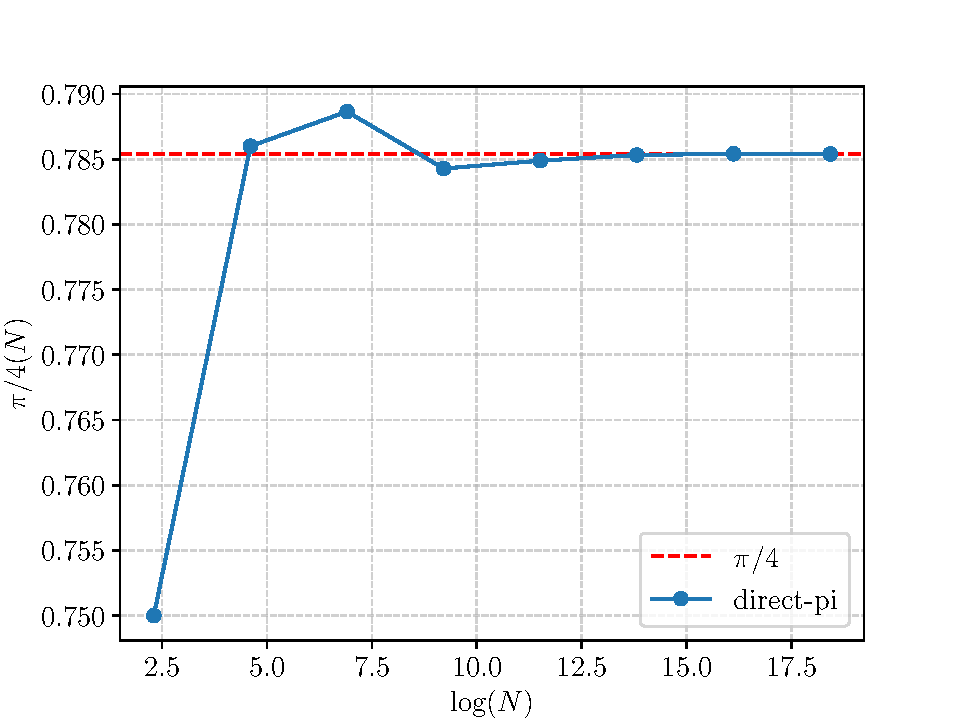
\includegraphics[width=0.8\textwidth]{p1/a/pi_q.pdf}
    \caption{Valor de $\pi/4$ para diferentes valores de $N$}
    \label{fig:p1_1}
\end{figure}
Al estar graficados para muchos valores de $N$, lo que hice fue 
promediar finalmente sobre todos los valores obtenidos para cada $N$.
Vemos que converge a $\pi/4$ para valores grandes de $N$. Esto al igual que otros métodos numéricos, se tiene que para poder acercarse al valor exacto de $\pi$, es necesario cada vez usar $N$ más grandes, esto nos habla 
de que para cuando $N \to \infty$ se tiene que el método debería llegar casi exactamente a $\pi/4$.
\par
Luego graficando la desviación cuadrática media,
\begin{figure}[H]
    \centering
    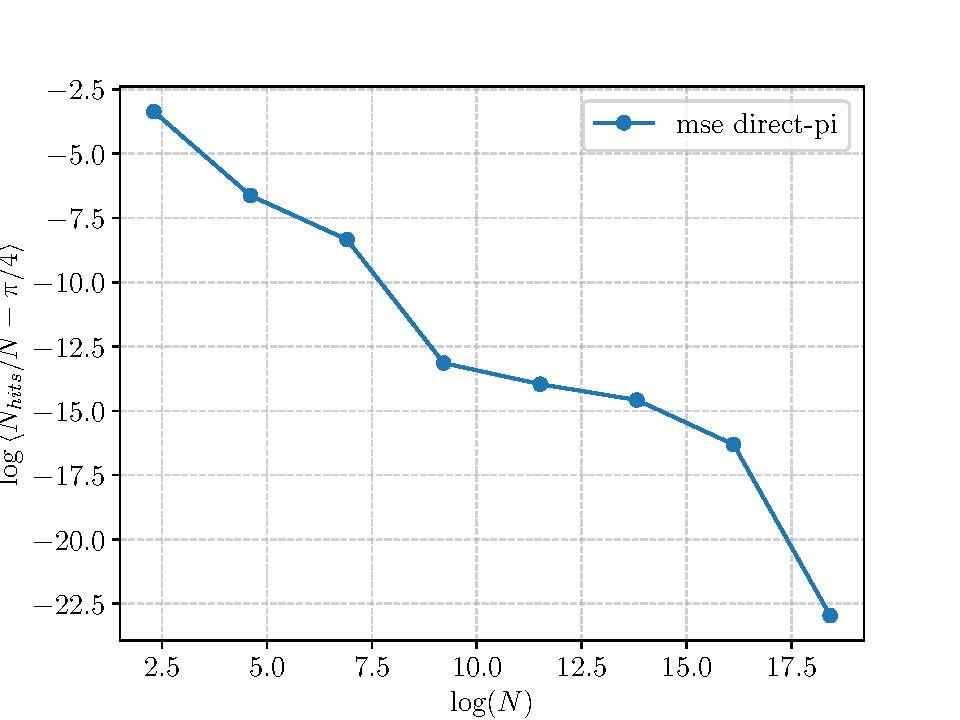
\includegraphics[width=0.8\textwidth]{p1/a/mse.pdf}
    \caption{Desviación cuadrática media para diferentes valores de $N$}
    \label{fig:p1_2}
\end{figure}
Donde al estar graficando en log-log al obtener un comportamiento casi lineal, vemos que la desviación cuadrática media decae de forma exponencial con $N$. 
Esto se hace evidente al pensar que para cuando se tienen valores de $N$ cada vez más grandes, estos se van acercando a $\pi/4$.
\subsection*{(b)}
Ahora usando el algoritmo de \texttt{markov-pi} podemos ver que nuevamente converge a $\pi/4$ para valores grandes de $N$.
\begin{figure}[H]
    \centering
    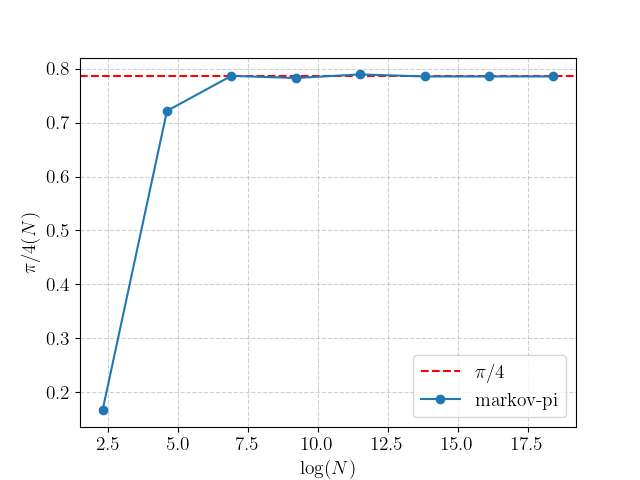
\includegraphics[width=0.8\textwidth]{p1/b/markov-pi.png}
    \caption{Valor de $\pi/4$ para diferentes valores de $N$ con $\delta = 0.3$ usando el método de Markov}
    \label{fig:p1_3}
\end{figure}
De este método, en comparación con el anterior, se observa que este converge más rápido hacía $\pi/4$ que el método de \texttt{direct-pi}.
Luego graficando la desviación cuadrática media, en función de $\delta $, con un $N = 10^{6}$ fijo con valores de $\delta \in [0,3]$,
\begin{figure}[H]
    \centering
    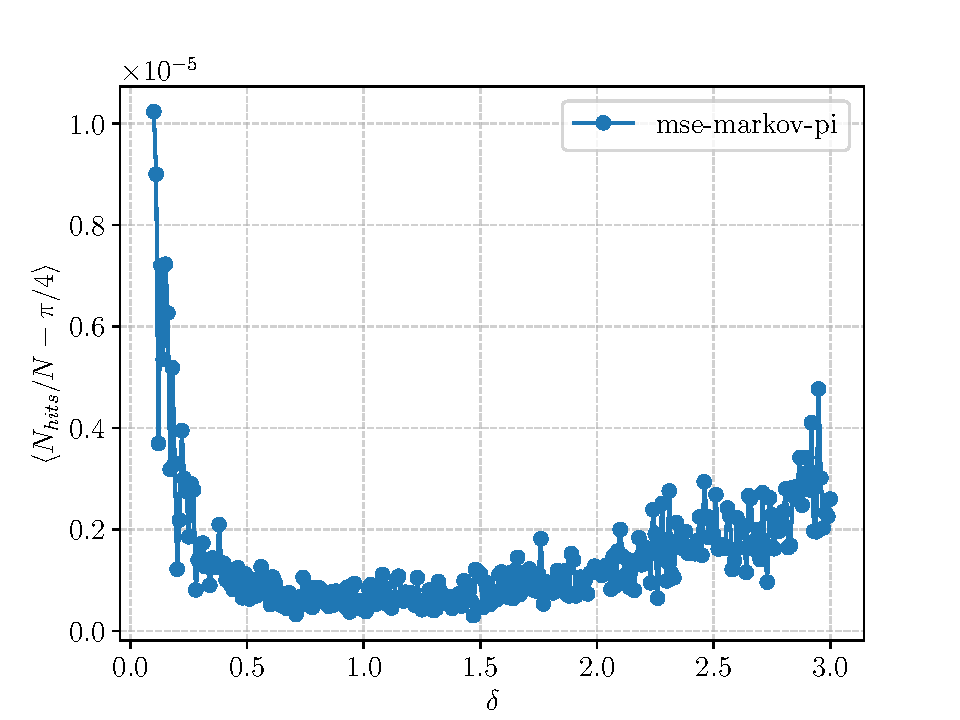
\includegraphics[width=0.8\textwidth]{p1/b/mse-markov.pdf}
    \caption{Desviación cuadrática media para diferentes valores de $\delta$}
    \label{fig:p1_4}
\end{figure}
Luego por último graficando la tasa de rechazo en función de $\delta$. Acá podemos observar que para valores pequeños de $\delta$ se obtiene una alta taza de aceptación casi entre $[\sim 0.3, \sim 1.5]$, donde además es posible observar que 
para valores más cercanos a $\delta = 3$, la tasa de rechazo, comienza a ser mucho mayor. Estos resultados son consistentes con lo planteado en clases (Clase 4 - Montecarlo).




\newpage
\section*{Pregunta 2}
\subsection*{(a)}   
Para este caso se tiene que usando el algoritmo \texttt{gray-flip} combinándolo con el algoritmo de \texttt{enumerate-ising} entonces de esta forma vemos que para $N = 2$, obtenemos,
usando condiciones de borde periódicas, los estados de,

\begin{figure}[H]
    \centering
    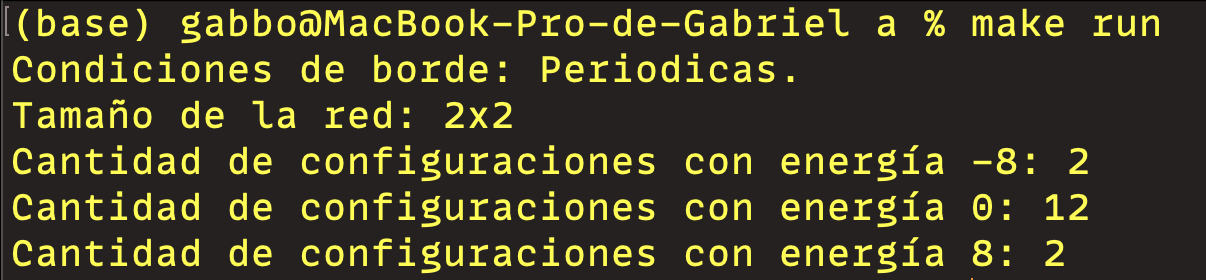
\includegraphics[width=0.8\textwidth]{p2/a/p2_1.png}
    \caption{Cantidad de configuraciones de energía para un sistema de $N=2$}
    \label{fig:p2_1}
\end{figure}
Luego para $N = 4$ obtenemos,
\begin{figure}[H]
    \centering
    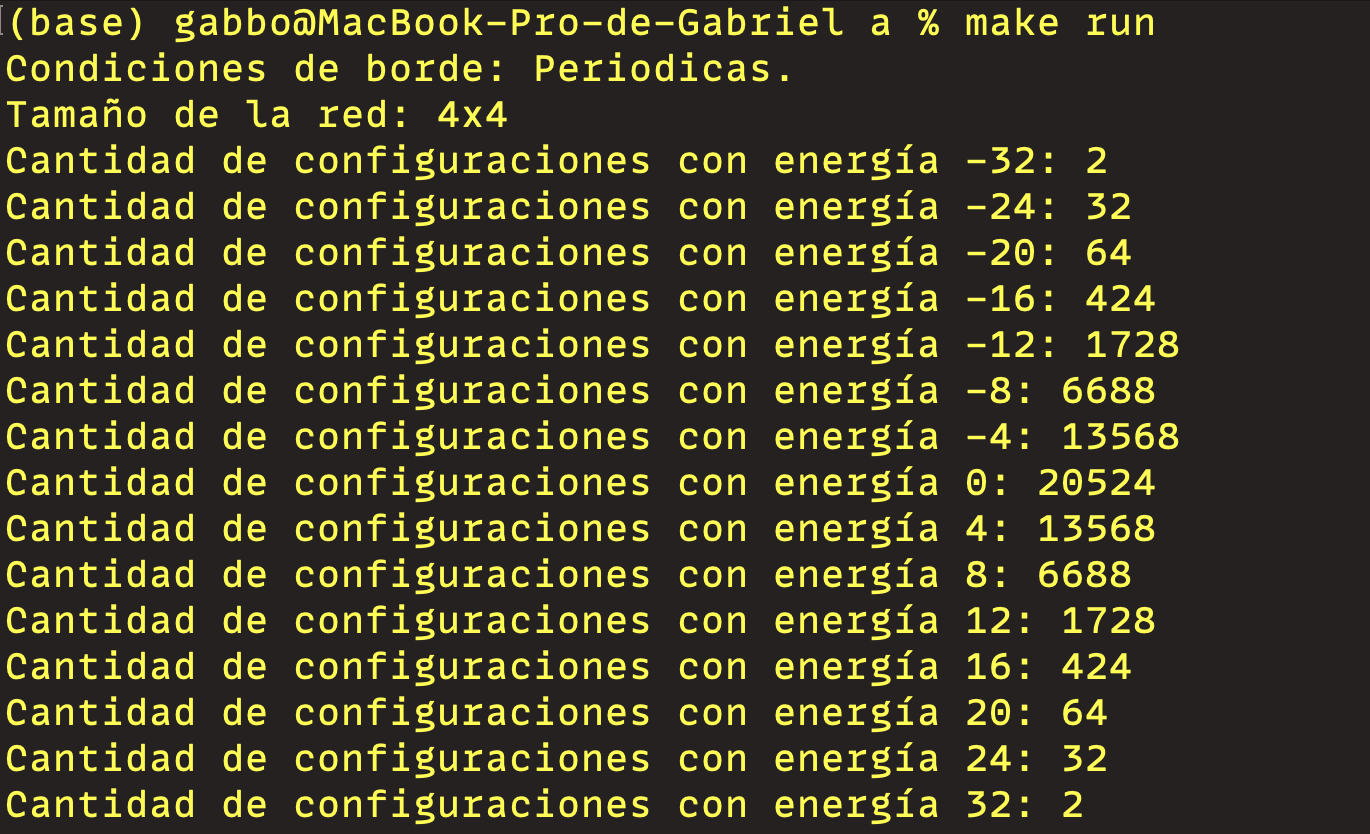
\includegraphics[width=0.8\textwidth]{p2/a/p2_2.png}
    \caption{Cantidad de configuraciones de energía para un sistema de $N=4$}
    \label{fig:p2_2}
\end{figure}
En ambos casos, es posible ver que se recupera la tabla de la diapositiva 15 de la clase 5. Es posible observar para estos casos, que existe una simetría en la cantidad de configuraciones de energía, esto se debe a que
para cada configuración de energía, existe una configuración de energía con la misma cantidad de energía pero con diferente configuración de spins. Entonces podemos representar $N(E) = N(-E)$
% Luego para $N = 6$ obtenemos,
% \begin{figure}[H]
%     \centering
%     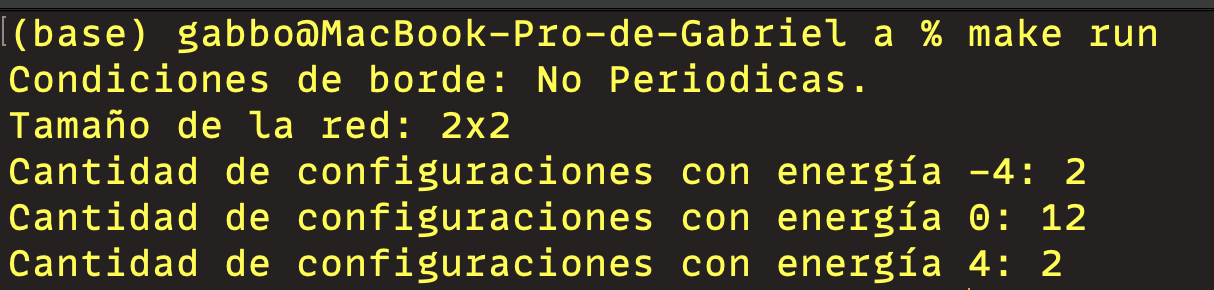
\includegraphics[width=0.8\textwidth]{p2/a/p2_3.png}
%     \caption{Cantidad de configuraciones de energía para un sistema de $N=6$}
%     \label{fig:p2_3}
% \end{figure}

Para condiciones de borde no periódicas, obtenemos
\begin{figure}[H]
    \centering
    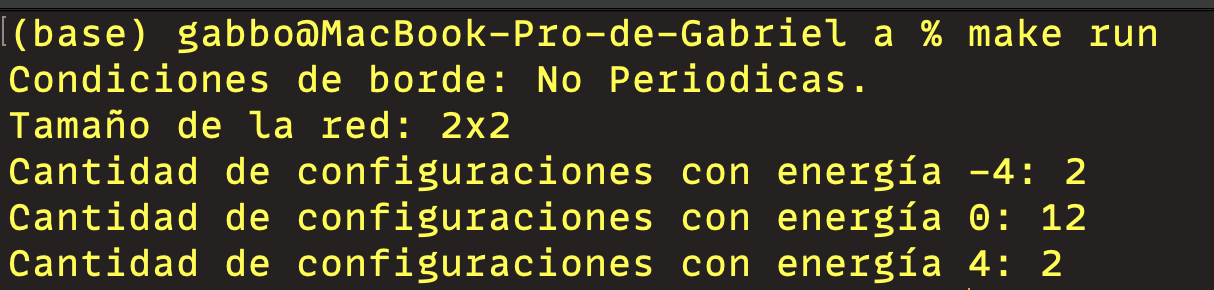
\includegraphics[width=0.8\textwidth]{p2/a/p2_3.png}
    \caption{Cantidad de configuraciones de energía para un sistema de $N=2$}
    \label{fig:p2_3}
\end{figure}
Para $N = 4$ obtenemos,
\begin{figure}[H]
    \centering
    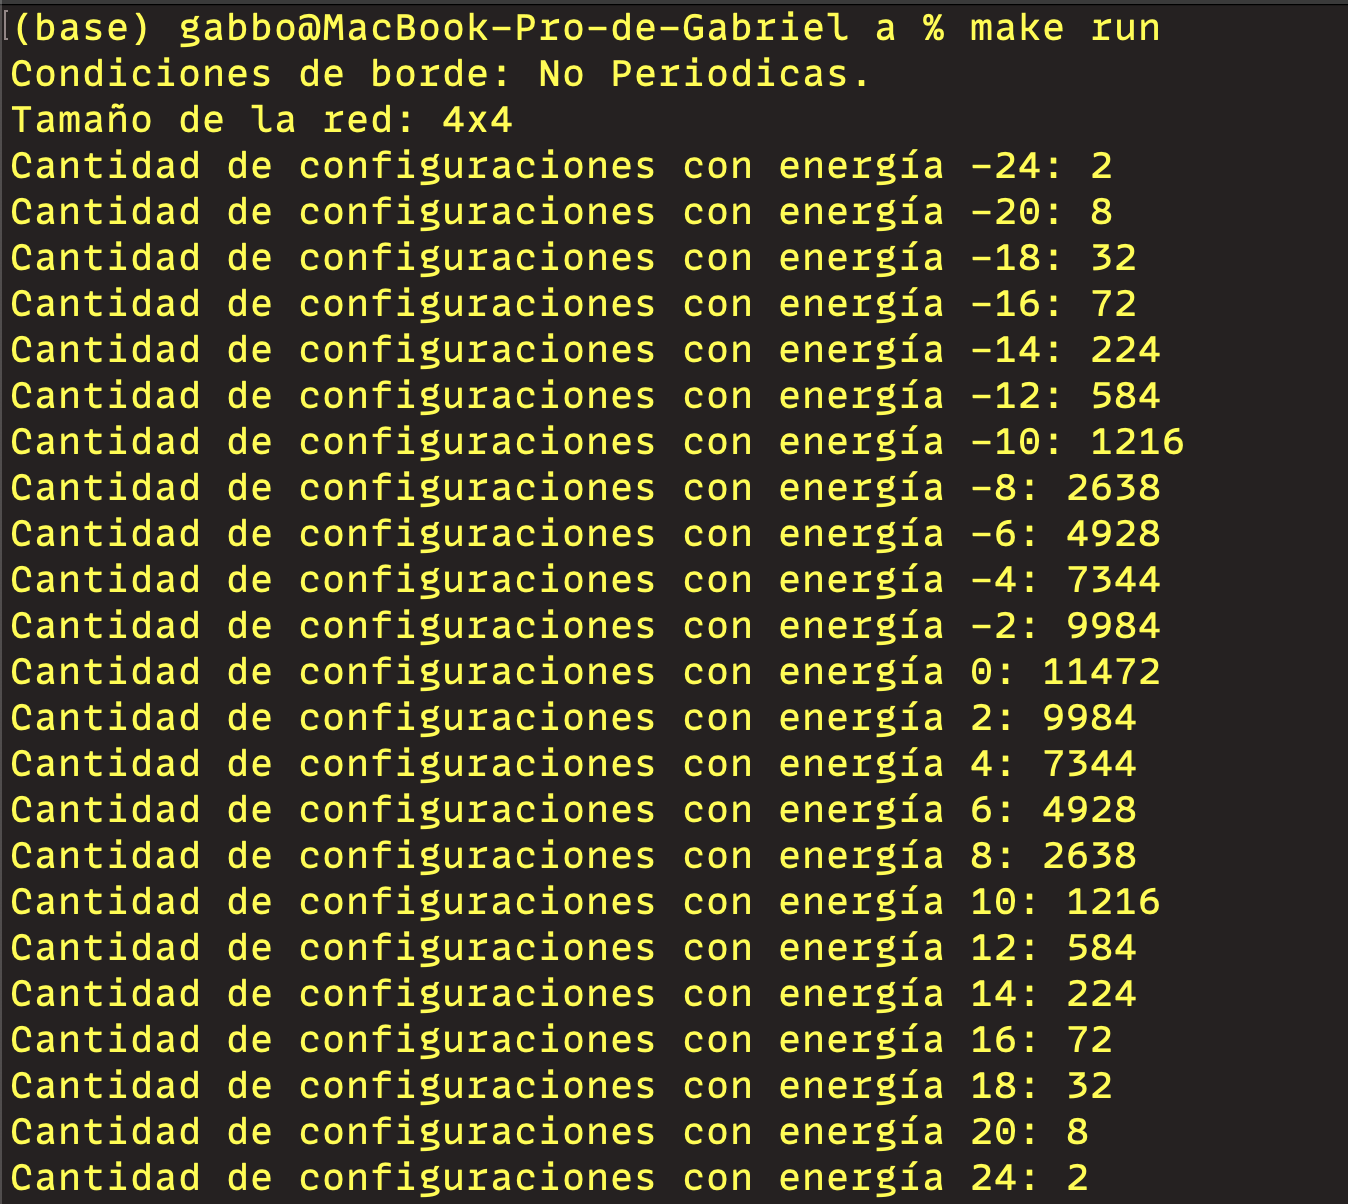
\includegraphics[width=0.8\textwidth]{p2/a/p2_4.png}
    \caption{Cantidad de configuraciones de energía para un sistema de $N=4$}
    \label{fig:p2_4}
\end{figure}
En este caso, al no tener condiciones de borde, es posible ver otras configuraciones de energía. 

\subsection*{(b)}

%%%%%%%%%%%%%%%%%%%%%%%%%%%%%%%%

\begin{figure}[H]
    \centering
    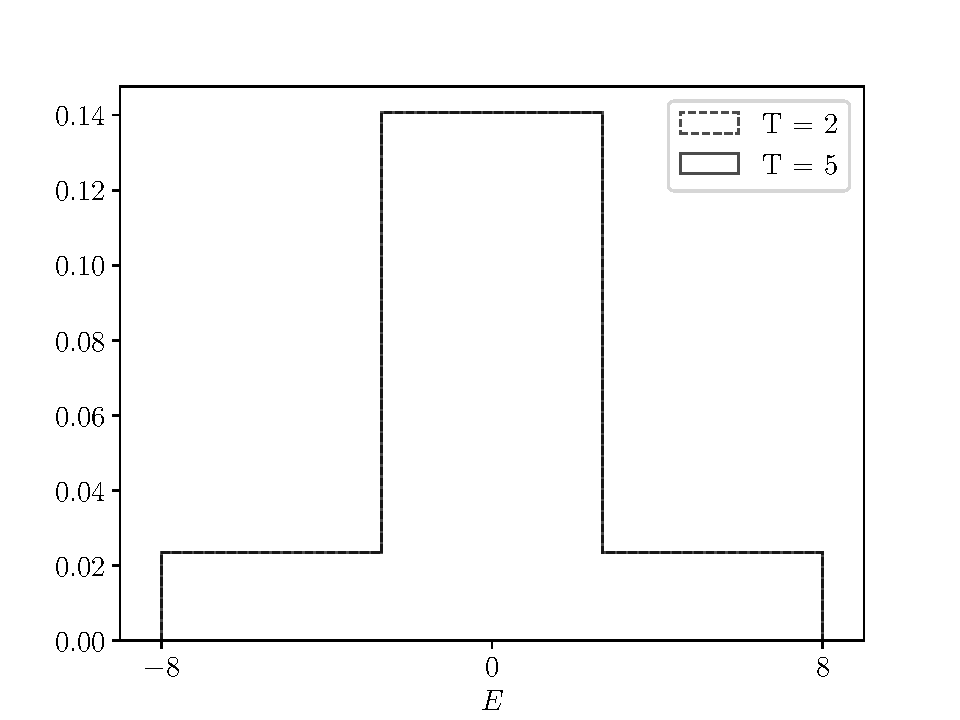
\includegraphics[width=0.8\textwidth]{p2/b/N2_energy_GrayFlip.pdf}
    \caption{Histograma de energía para un sistema de $N=2$}
    \label{fig:p2_4}
\end{figure}

\begin{figure}[H]
    \centering
    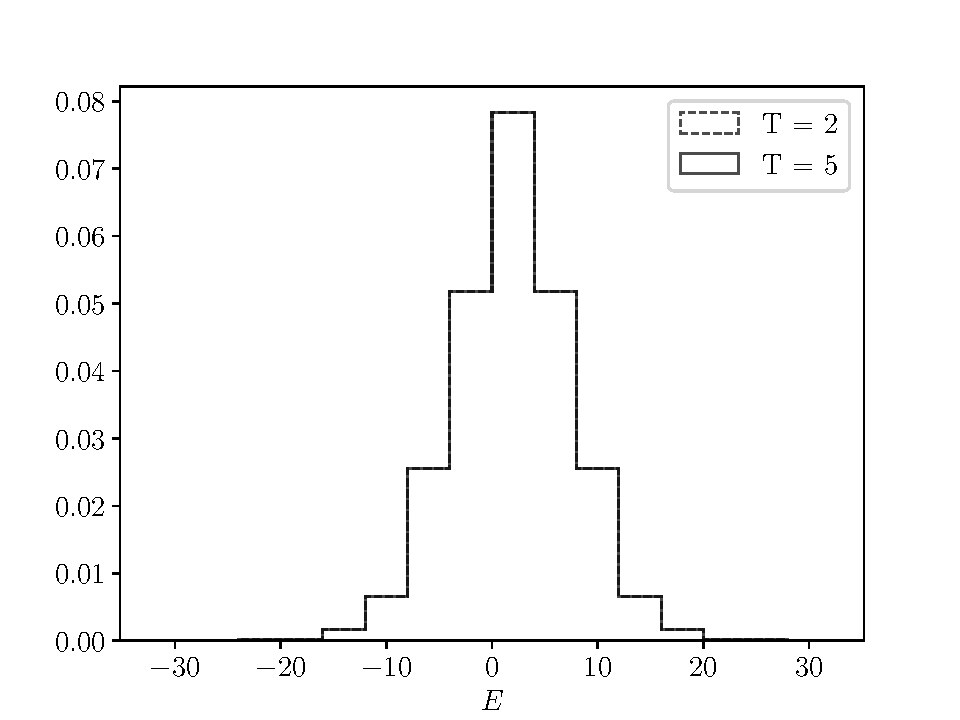
\includegraphics[width=0.8\textwidth]{p2/b/N4_energy_GrayFlip.pdf}
    \caption{Histograma de energía para un sistema de $N=4$}
    \label{fig:p2_4}
\end{figure}

\begin{figure}[H]
    \centering
    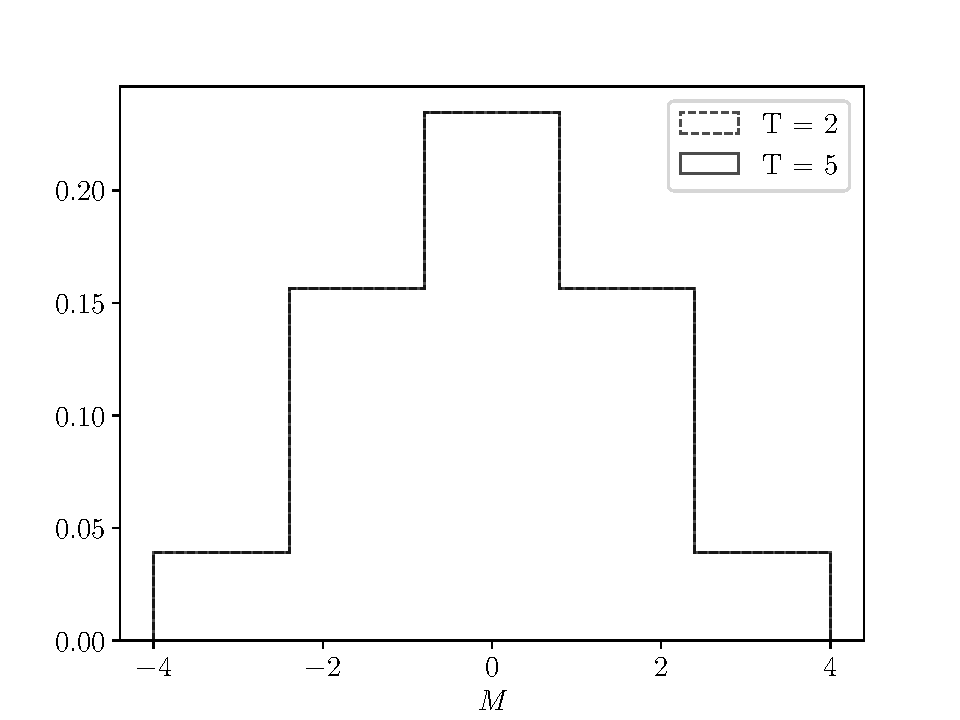
\includegraphics[width=0.8\textwidth]{p2/b/N2_magnetizacion_GrayFlip.pdf}
    \caption{Histograma de magnetización para un sistema de $N=2$}
    \label{fig:p2_5}
\end{figure}

\begin{figure}[H]
    \centering
    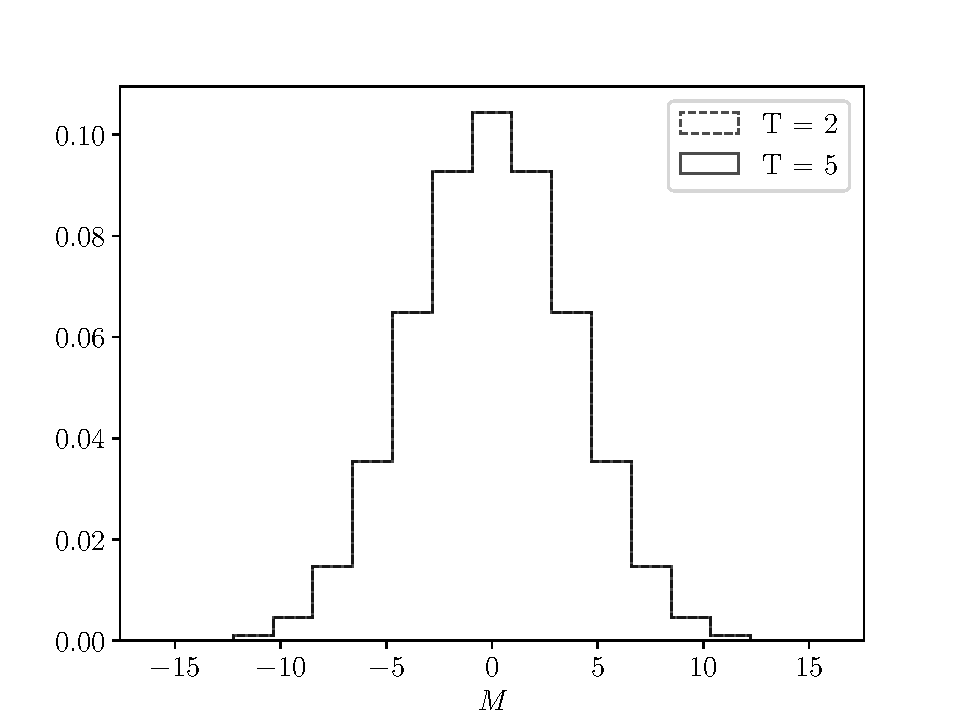
\includegraphics[width=0.8\textwidth]{p2/b/N4_magnetizacion_GrayFlip.pdf}
    \caption{Histograma de magnetización para un sistema de $N=4$}
    \label{fig:p2_6}
\end{figure}

\begin{figure}[H]
    \centering
    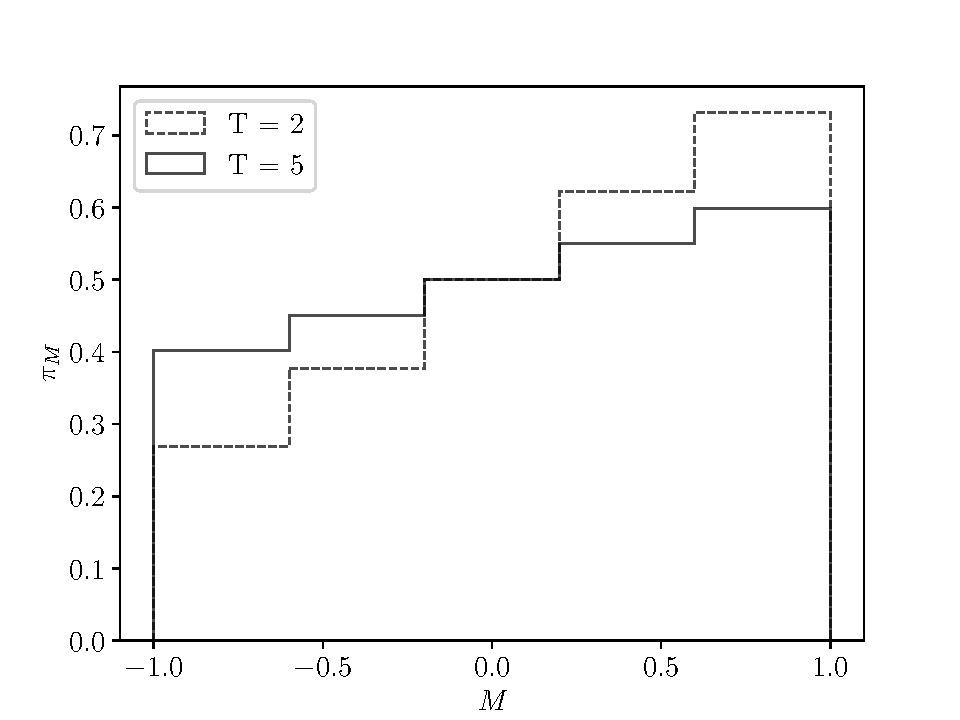
\includegraphics[width=0.8\textwidth]{p2/b/N2_pi_m.pdf}
    \caption{Histograma de $\pi_M$ para un sistema de $N=2$}
    \label{fig:p2_6}
\end{figure}

\begin{figure}[H]
    \centering
    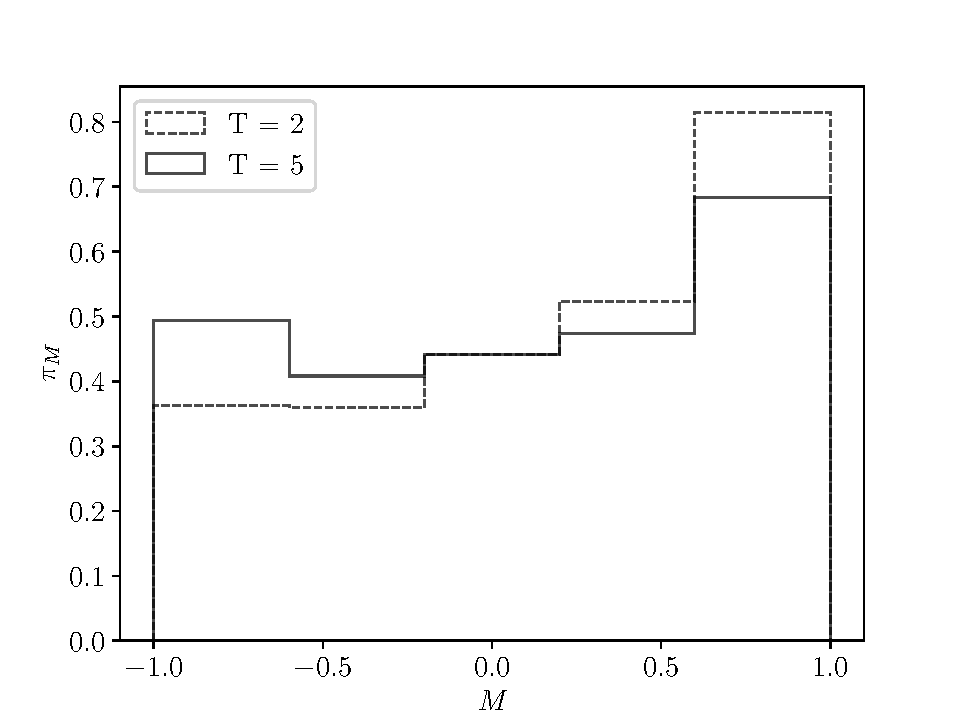
\includegraphics[width=0.8\textwidth]{p2/b/N4_pi_m.pdf}
    \caption{Histograma de $\pi_M$ magnetización para un sistema de $N=4$}
    \label{fig:p2_6}
\end{figure}

Luego el binder cumulant para $N = 2$ es,
\begin{figure}[H]
    \centering
    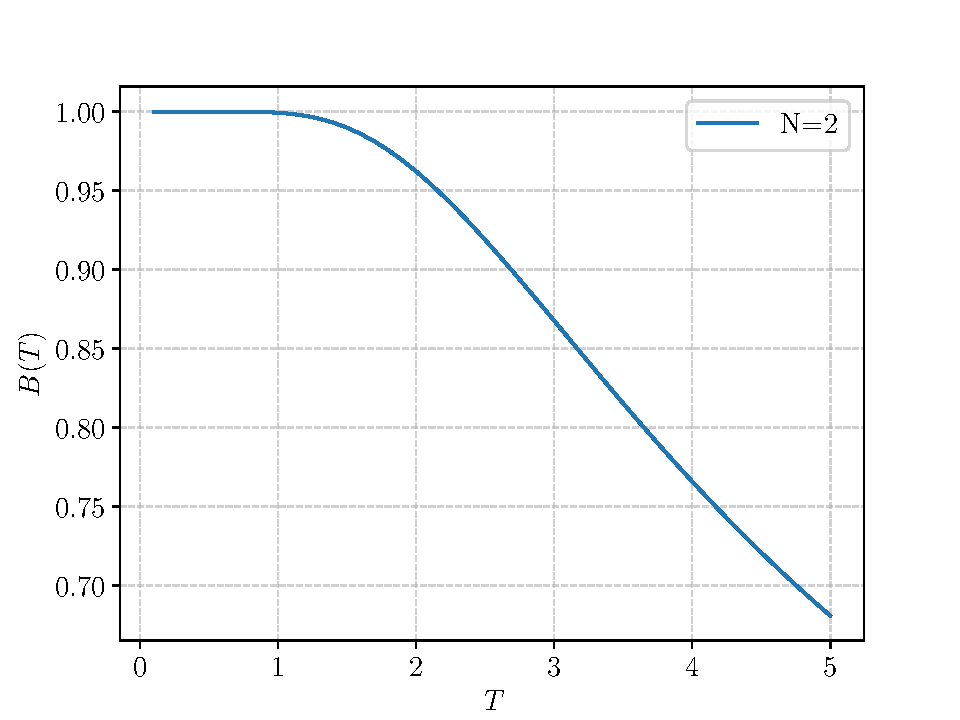
\includegraphics[width=0.8\textwidth]{p2/N2_binder.pdf}
    \caption{Binder cumulant para un sistema de $N=2$}
    \label{fig:p2_7}
\end{figure}

\begin{figure}[H]
    \centering
    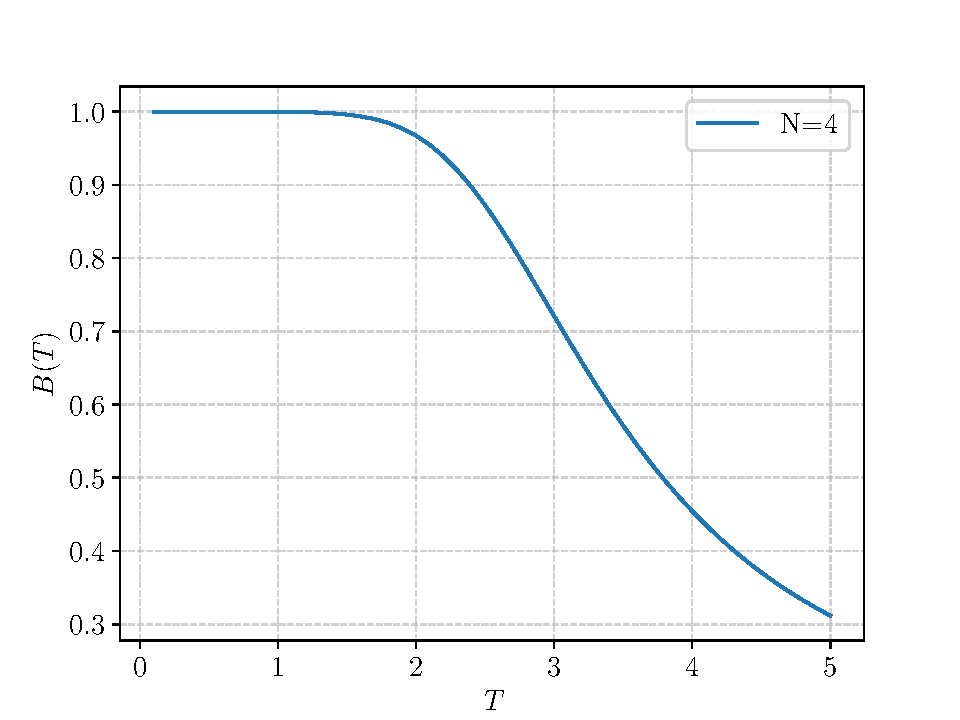
\includegraphics[width=0.8\textwidth]{p2/N4_binder.pdf}
    \caption{Binder cumulant para un sistema de $N=4$}
    \label{fig:p2_8}
\end{figure}
Podemos ver que el Binder Cumulant, casi intersectan en $T_c = 2/\ln{(1+\sqrt{2})}$, lo que es consistente con lo esperado.
\begin{figure}[H]
    \centering
    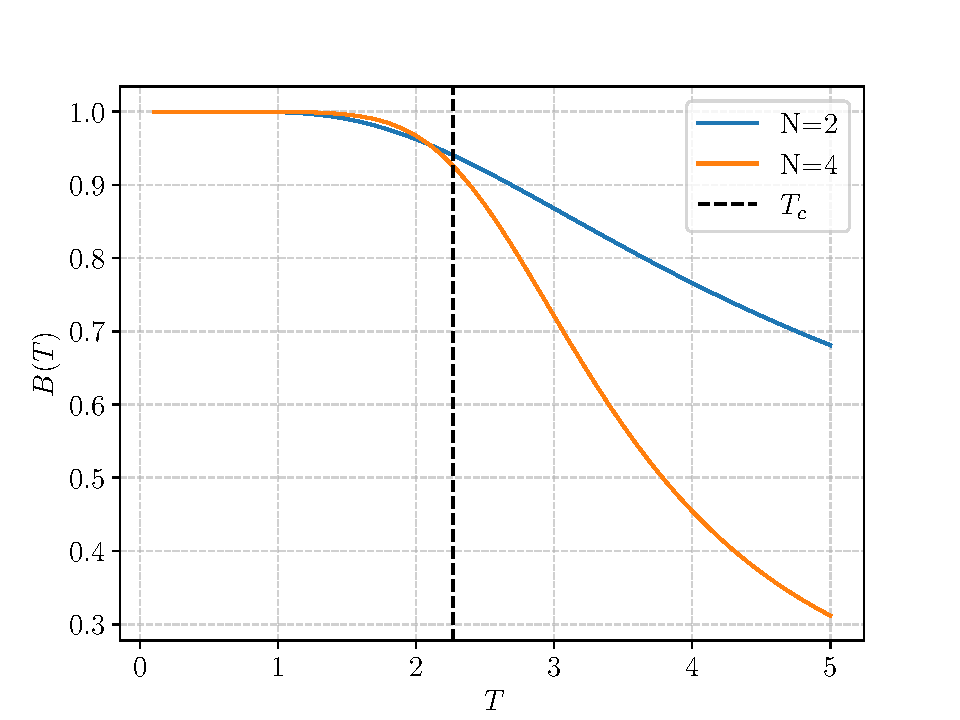
\includegraphics[width=0.8\textwidth]{p2/all_binder.pdf}
    \caption{Binder cumulant para 2 redes de $N=2$ y $N=4$}
    \label{fig:p2_8}
\end{figure}
Es posible observar que las curvas de Binder Cumulant, tienen valores donde ambas curvas coinciden, pero esto se me ocurre que tenga que ver con los comportamientos modal y bimodal, 
ahora esto, ocurre cercano a temperaturas a $T_c = 2/\ln{(1+\sqrt{2})}$. Esto porque para el minuto en el que hice esta pregunta ya había hecho la pregunta 4, donde en los histogramas Para
$T = 2$ existía un comportamiento bimodal y justamente para $T = 5$ hay un comportamiento unimodal, donde según las clases en el punto $T_c$ es justamente la cota donde ocurre un comportamiento o el otro. 


\newpage
\section*{Pregunta 3}
Entonces para este caso, tenemos que usando el algoritmo de \texttt{markov-ising} o \texttt{Metropolis}. Podemos calcular la energía y el calor específico como función de la temperatura para un red de $N = 6$.
Usando condiciones de borde periódicas de esta forma podemos obtener los resultados según la figura \ref{fig:p3_1}
\begin{figure}[H]
    \centering
    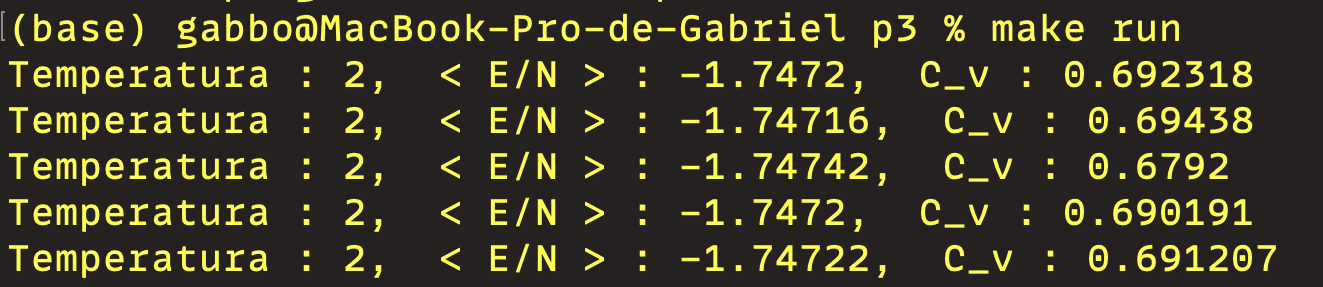
\includegraphics[width=0.8\textwidth]{p3/p3_1.png}
    \caption{Energía y calor específico como función de la temperatura para una red de $N = 6$ para temperatura fija T = 2 y $10^6$ Sampling Steps.}
    \label{fig:p3_1}
\end{figure}
Donde notamos que comparando con la figura \ref{fig:p3_2} obtenida desde la diapositiva 23 de la clase 5 podemos ver que los resultados son consistentes.
\begin{figure}[H]
    \centering
    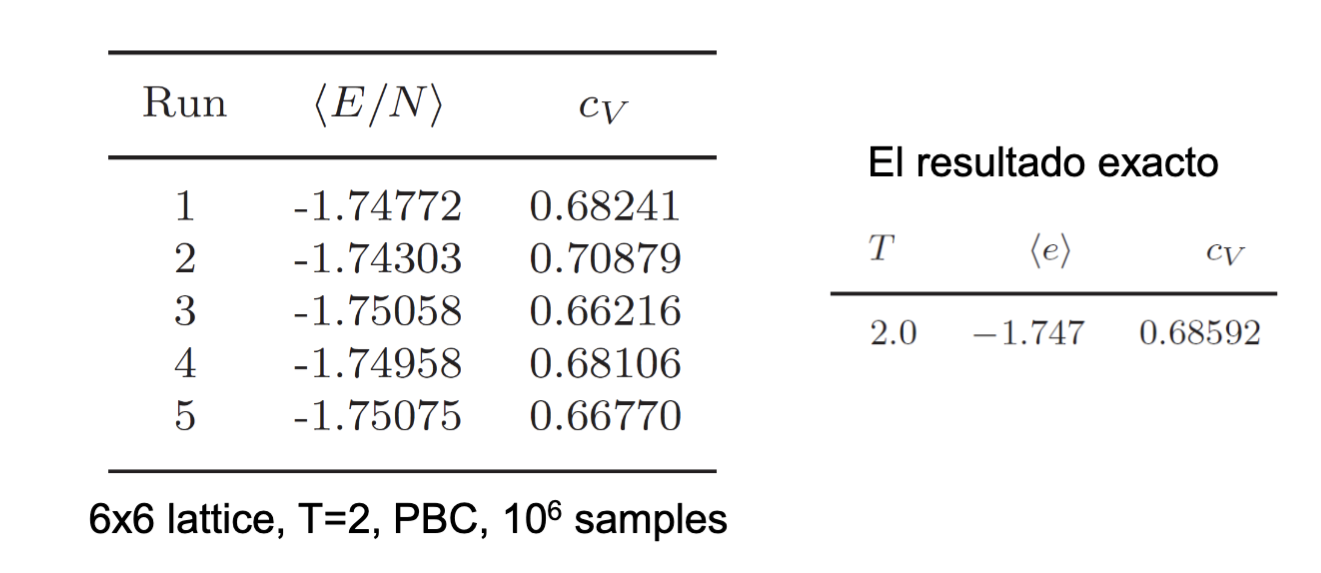
\includegraphics[width=0.8\textwidth]{p3/p3_2.png}
    \caption{Energía y calor específico como función de la temperatura para una red de $N = 6$ para temperatura fija T = 2. Valores de referencias rescatados desde la clase.}
    \label{fig:p3_2}
\end{figure}
De hecho dentro de los primeros 4 decimales, este método corresponde a una buen aproximación al sistema. Para poder obtener una mejor aproximación, es necesario obtener más runs.
Además, es necesario hacer una fase de equilibración antes de calcular la energía promedio. Esto ya que es necesario tener una fase donde al igual que antes hagamos iteraciones del sistema para 
acercarnos al equilibrio (o valor real) debido a la aleatoriedad del proceso. \\
Por esto último de hecho es que se obtienen diferentes valores para la energía en el orden del cuarto decimal en comparación con la figura \ref{fig:p3_2}. 


Luego graficando la magnetización absoluta promedio como función de la temperatura para una red de $N = 6$ tomando $10^6$ Sampling Steps. Obtenemos la figura \ref{fig:p3_3}
\begin{figure}[H]
    \centering
    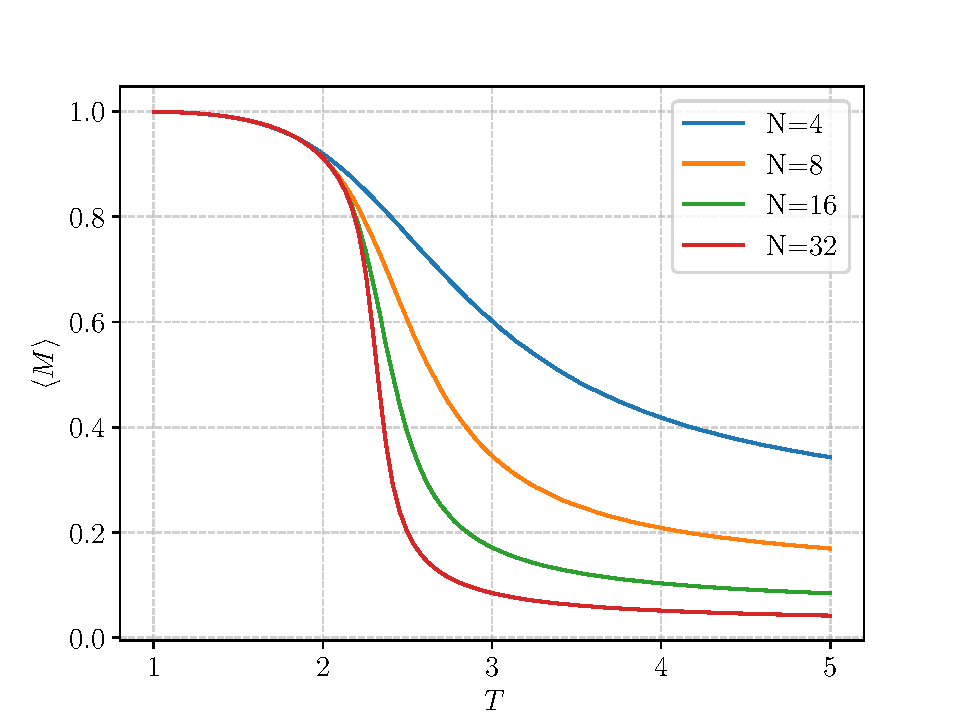
\includegraphics[scale=0.65]{p3/T_vs_M.pdf}
    \caption{Magnetización absoluta promedio como función de la temperatura para una red de $N = 6$ para temperatura fija T = 2}
    \label{fig:p3_3}
\end{figure}
Al graficar la magnetizacion contra la temperatura es posible observar que a temperaturas cercanas a $[0,1] $, se tiene que la magnetización es constante. Esto se debe a que estamos cercano al 0 de temperatura,
otras teorías deberían ser válidas en los límites para cuando $T>> 1$ o similares, pero deberiamos ver otros efectos y quizás la magnetización se podría no visualizar de manera completa. 
\par
Además es posible observar que para cuando mientras más grande es nuestra red de spines, más sensible es la magnetización a los cambios de temperatura, esto lo vemos en las curvas para cuando $N > 4$ donde cercano al punto de $T \approx 2.2$, la 
magnetización decae de forma significativa, siendo mientras más grande la red, esta decae más rápido.

\newpage
\section*{Pregunta 4}
Usando el algoritmo de \texttt{cluster-ising}, podemos ver que podemos recuperar los valores para la energía y calor específico, 
\begin{figure}[H]
    \centering
    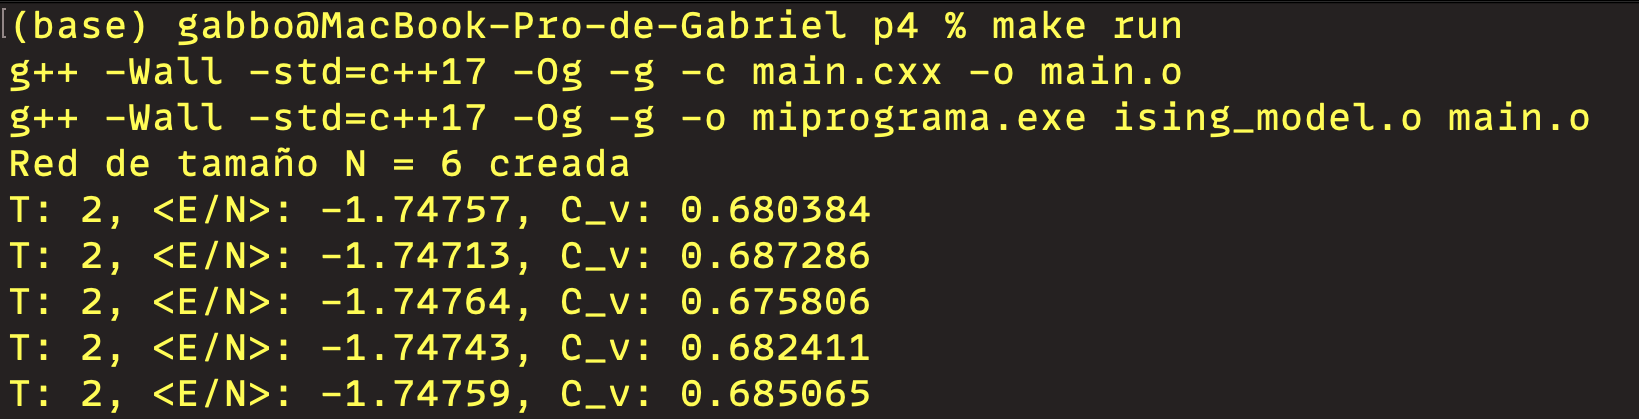
\includegraphics[width=0.8\textwidth]{p4/p4_1.png}
    \caption{Energía y calor específico como función de la temperatura para una red de $N = 6$ para temperatura fija T = 2 y $10^6$ Sampling Steps.}
    \label{fig:p4}
\end{figure}
Es posible comparando los resultados nuevamente usando un tiempo de equilibración y calculando la energía poder recuperar los resultados casi exactos de la figura \ref{fig:p3_2}, pero usando ahora el método de \texttt{cluster-ising}, con 
la diferencia que para este método podemos llegar a resultados más exactos en los runs que hicimos, donde nos acercamos cada vez más al resultado de $C_v = 0.685$, pero al ser un método con cierto grado de aleatoriedad y necesitar un tiempo de equilibrio, mientras 
nayor sea el tiempo de equilibrio y mayor el número de runs, más deberíamos acércanos a los valores exactos.

Ahora obteniendo los histogramas de magnetización, tenemos que para $N=6$,
\begin{figure}[H]
    \centering
    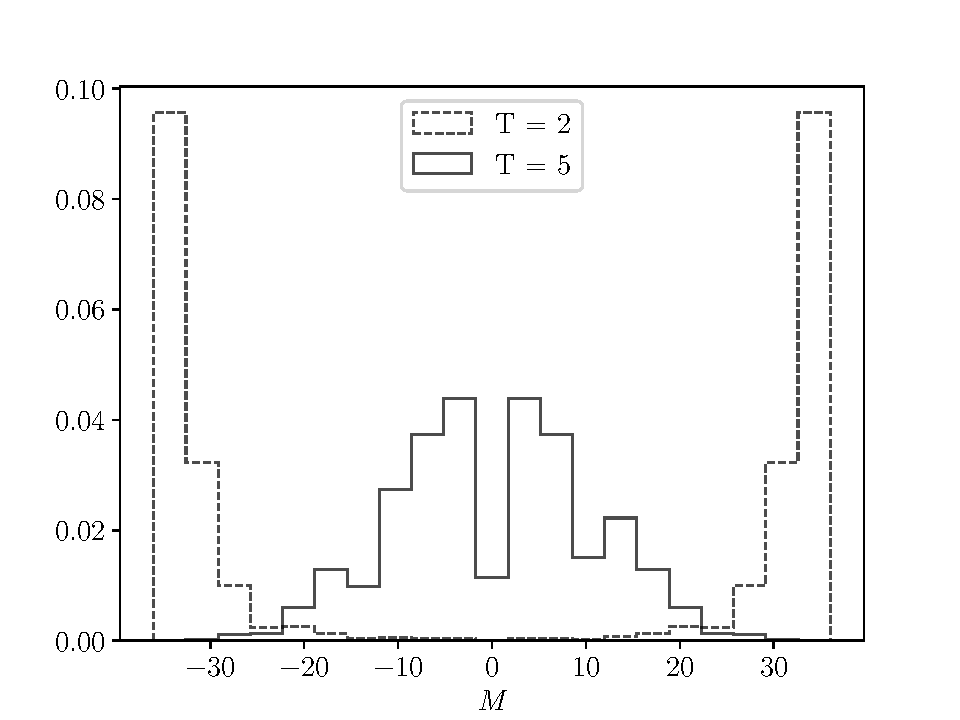
\includegraphics[width=0.8\textwidth]{p4/N6_magnetization_hist.pdf}
    \caption{Histograma de magnetización para una red de $N = 6$}
    \label{fig:p4_1}
\end{figure}

Luego para $N= 16$,
\begin{figure}[H]
    \centering
    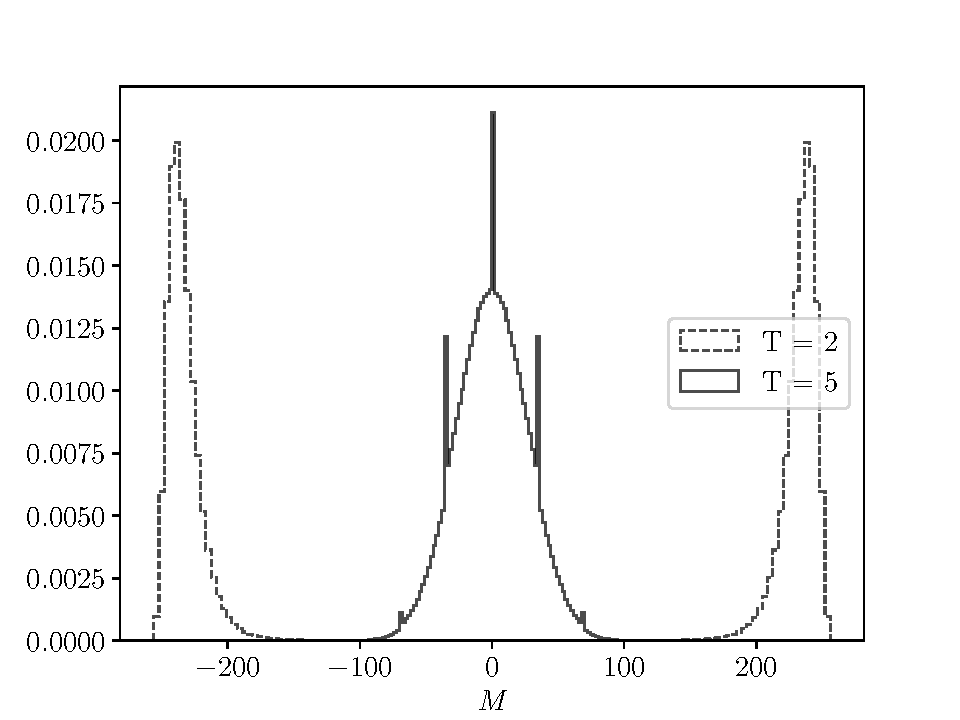
\includegraphics[width=0.8\textwidth]{p4/N16_magnetization_hist.pdf}
    \caption{Histograma de magnetización para una red de $N = 16$}
    \label{fig:p4_2}
\end{figure}
\newpage
Luego para $N= 32$,
\begin{figure}[H]
    \centering
    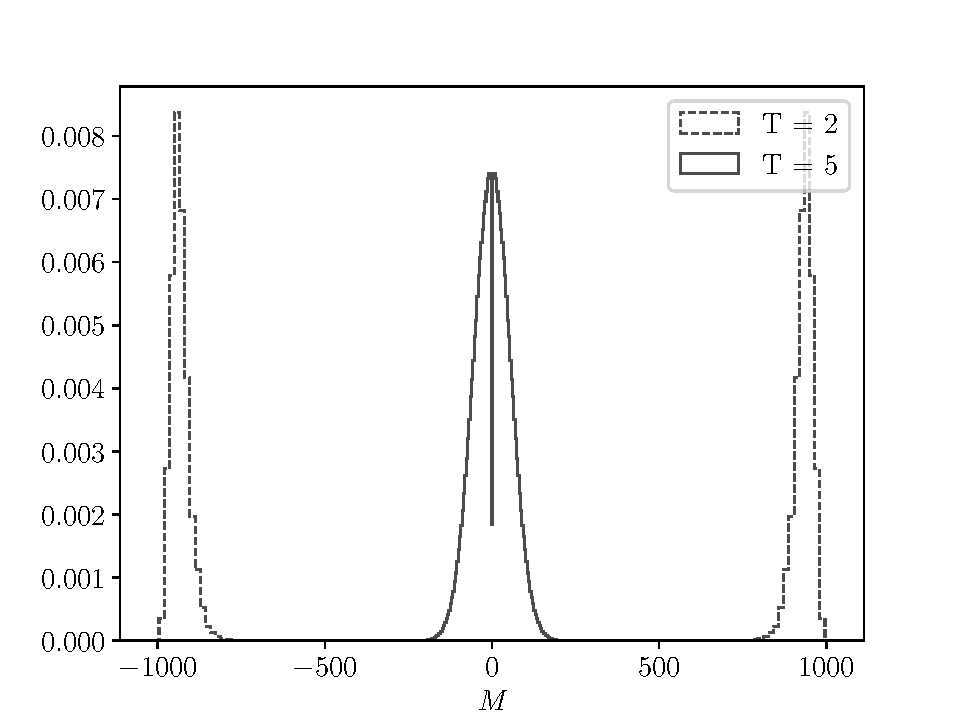
\includegraphics[width=0.8\textwidth]{p4/N32_magnetization_hist.pdf}
    \caption{Histograma de magnetización para una red de $N = 32$}
    \label{fig:p4_3}
\end{figure}

Luego para $N= 64$,
\begin{figure}[H]
    \centering
    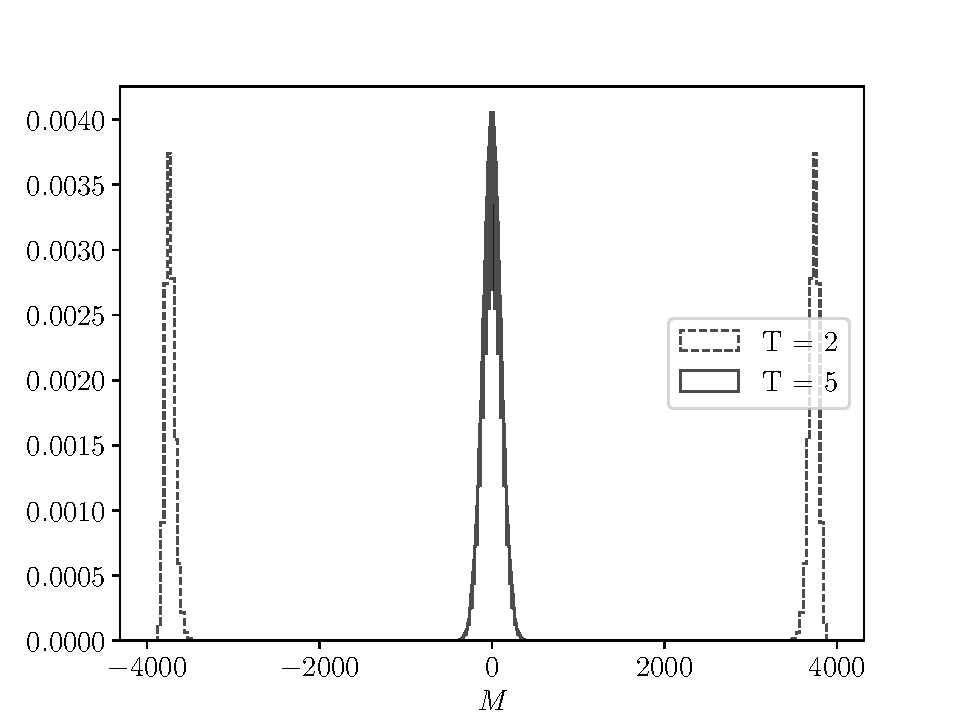
\includegraphics[width=0.8\textwidth]{p4/N64_magnetization_hist.pdf}
    \caption{Histograma de magnetización para una red de $N = 64$}
    \label{fig:p4_4}
\end{figure}

En los histogramas es posible ver que para todas las redes al graficar $T = 2$ y $T = 5$, existe un comportamiento bimodal y unimodal respectivamente. 
Esto es consistente con lo visto a través del binder cumulant de la pregunta 2. Se puede inferir nuevamente que entre $T = 2$ y $T = 5$ existe un punto crítico donde se pasa de un comportamiento bimodal a unimodal.
Graficando los binder cumulant para diferentes tamaños de red,
\begin{figure}[H]
    \centering
    \begin{minipage}{0.45\textwidth}
        \centering
        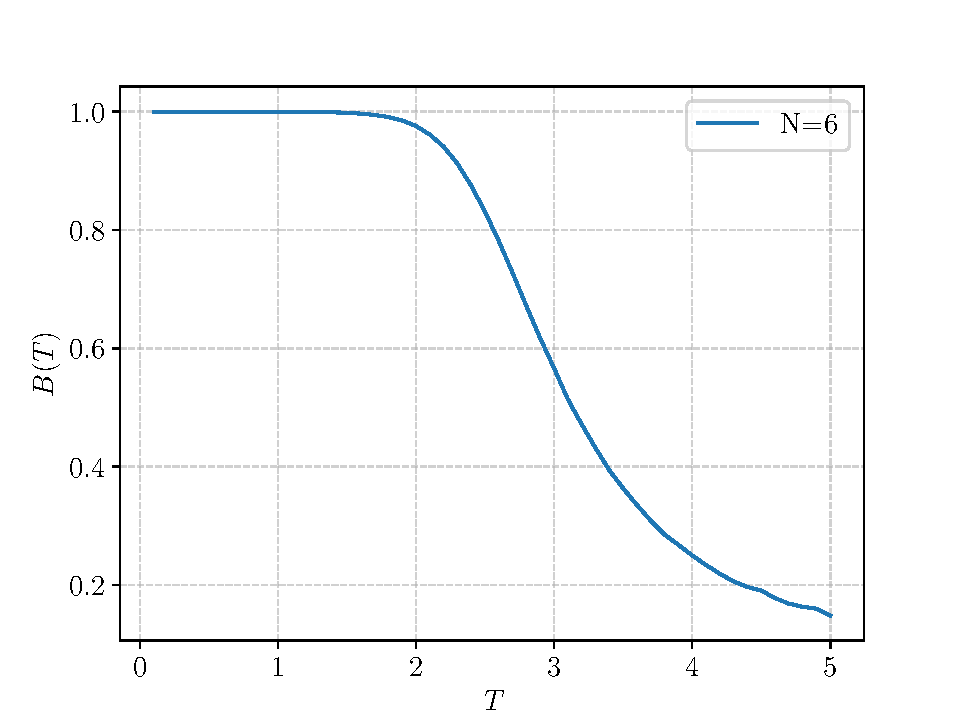
\includegraphics[width=\textwidth]{p4/N6_binder.pdf}
        \caption{Binder cumulant para una red de $N = 6$}
        \label{fig:p4_5}
    \end{minipage}
    \hfill
    \begin{minipage}{0.45\textwidth}
        \centering
        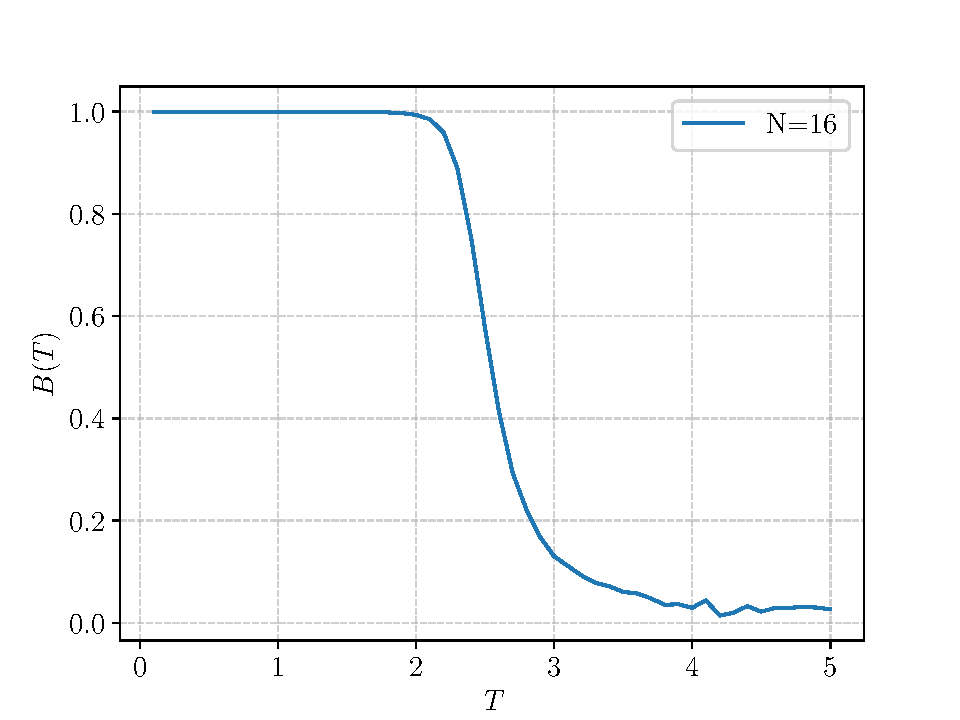
\includegraphics[width=\textwidth]{p4/N16_binder.pdf}
        \caption{Binder cumulant para una red de $N = 16$}
        \label{fig:p4_6}
    \end{minipage}
    \vfill
    \begin{minipage}{0.45\textwidth}
        \centering
        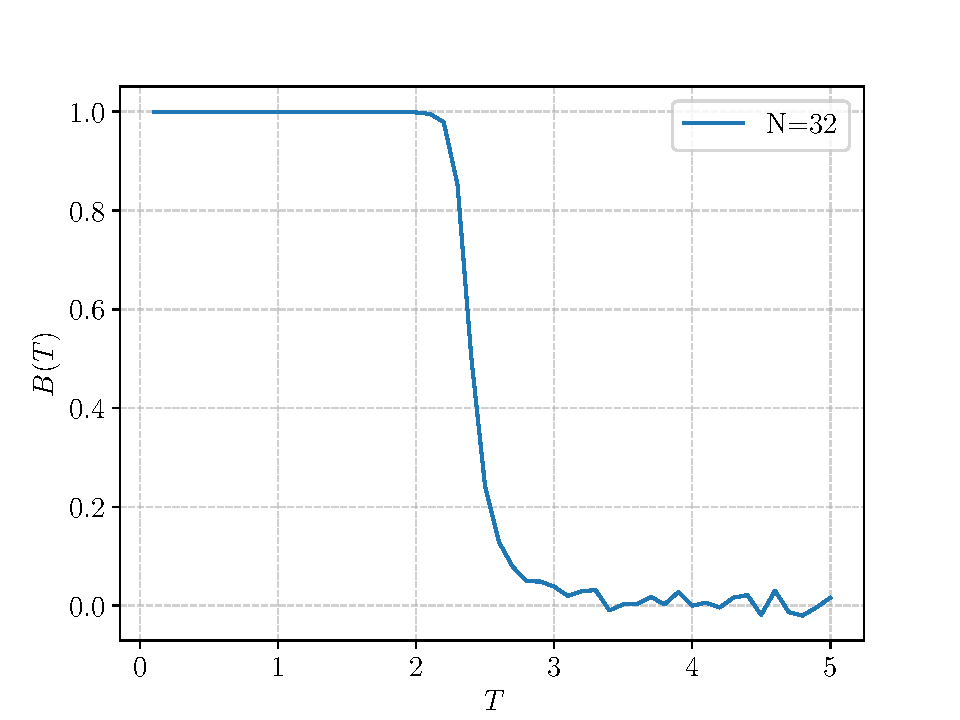
\includegraphics[width=\textwidth]{p4/N32_binder.pdf}
        \caption{Binder cumulant para una red de $N = 32$}
        \label{fig:p4_7}
    \end{minipage}
    \hfill
    \begin{minipage}{0.45\textwidth}
        \centering
        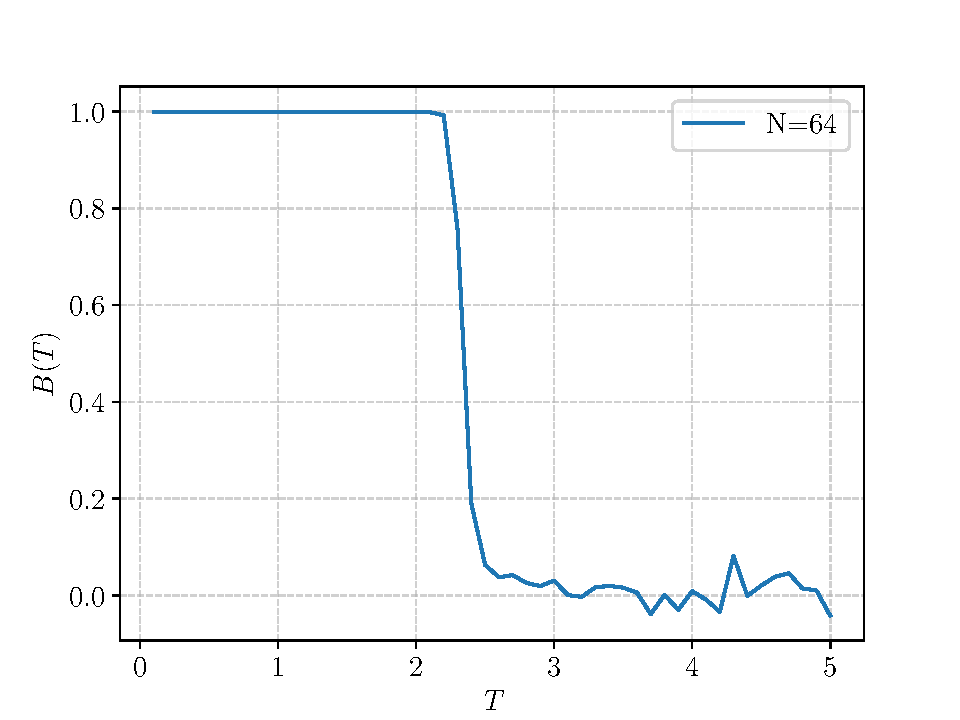
\includegraphics[width=\textwidth]{p4/N64_binder.pdf}
        \caption{Binder cumulant para una red de $N = 64$}
        \label{fig:p4_8}
    \end{minipage}
\end{figure}
Graficando todas las curva dentro de un mismo canvas, es posible ver que estos intersectan casi en $T_c = 2/\ln{(1+\sqrt{2})}$, según,
\begin{figure}[H]
    \centering
    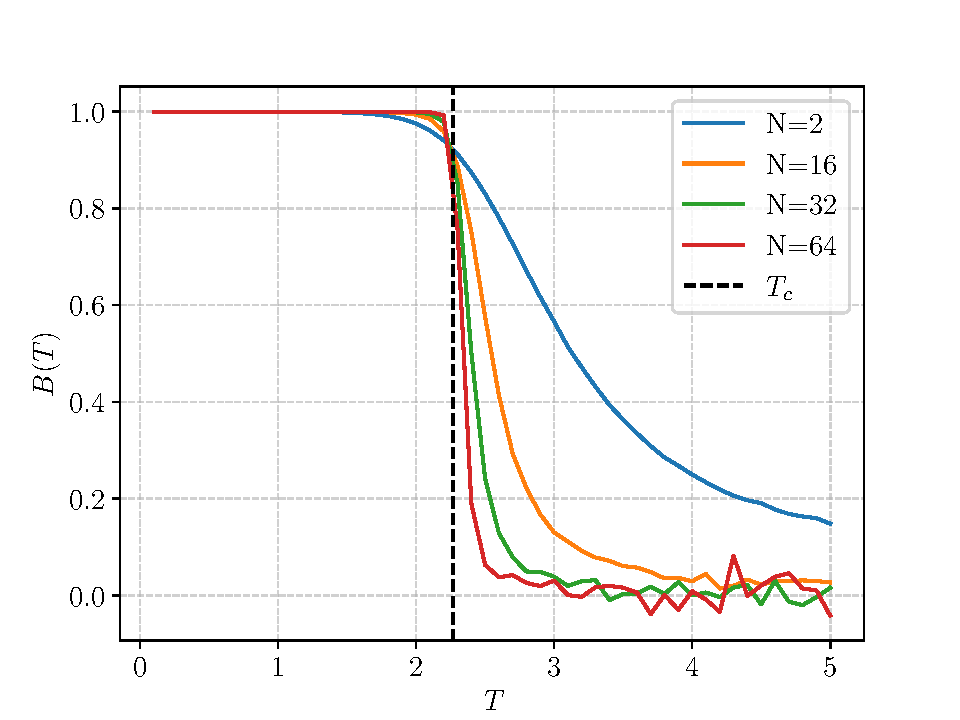
\includegraphics[width=0.65\textwidth]{p4/all_binder.pdf}
    \caption{Binder cumulant para diferentes tamaños de red}
    \label{fig:p4_9}
\end{figure}
Podemos inferir que justamente es en $T_c$ donde los comportamientos unimodal y bimodal son críticos y existe alguna transición entre ellos. 

% \newpage
% \hfill
% \begin{center}
%     \Huge \textbf{Códigos}
% \end{center}
% \newpage
% \section*{Pregunta 1}
% \subsection*{(a)}
% \begin{lstlisting}[language=C++]
% #include <iostream>
% #include <fstream> // Para manejar archivos
% #include <cstdlib> // Para rand() y srand()
% #include <ctime>   // Para time()
% #include <cmath>
% #include <vector>  

% // Funcion que genera numeros random.
% double random_uniform(double min, double max) {
%     return min + static_cast<double>(rand()) / (static_cast<double>(RAND_MAX) / (max - min));
% }

% // Funcion que calcula el valor de pi.
% int direct_pi(int N) {
%     int n_hits = 0;
%     for (int i = 0; i < N; ++i) {
%         double x = random_uniform(-1.0, 1.0);
%         double y = random_uniform(-1.0, 1.0);
%         if (( (x * x) + (y * y ) ) < 1.0){
%             ++n_hits;
%         }
%     }
%     return n_hits;
% }

% // Funcion que calcula la desviacion cuadratica media (MSE)
% double compute_mse(const std::vector<double>& pi_estimates, double pi_4) {
%     double mse = 0.0;
%     int num_runs = pi_estimates.size();
    
%     for (int i = 0; i < num_runs; ++i) {
%         double diff = pi_estimates[i] - pi_4;
%         mse += diff * diff;
%     }
    
%     return mse / num_runs;  // Retorna el promedio de las diferencias al cuadrado
% }

% int main() {
%     srand(time(0)); // Inicializa la semilla para rand()
%     std::ofstream output_pi;
%     output_pi.open("direct_pi.dat");
%     for (int exp = 1; exp <= 8; ++exp) {
%         int N = static_cast<int>(pow(10, exp));
%         for (int i = 0; i < 20; ++i) {
%             int hits = direct_pi(N);
%             double pi_estimate =  (double)hits / N; // pi/4
%             output_pi << N << " " << pi_estimate << std::endl;
%         }
%     }
%     output_pi.close();

%     std::ofstream output_mse;
%     output_mse.open("mse_direct_pi_1.dat");
%     for (int exp = 1; exp <= 8; ++exp) {
%         int N_fixed = static_cast<int>(pow(10, exp));
%         const int runs = 20;
%         const double pi_4 = M_PI / 4.0;
%         std::vector<double> pi_estimates;
%         for (int i = 0; i < runs; ++i) {
%             int hits = direct_pi(N_fixed);
%             double pi_estimate = (double)hits / N_fixed;
%             pi_estimates.push_back(pi_estimate);
%         double mse = compute_mse(pi_estimates, pi_4);
%         output_mse << N_fixed << " " << mse << std::endl;
%         std::cout << N_fixed << " " << mse << std::endl;
%         }
%     }
%     return 0;
% }
% \end{lstlisting}

% \subsection*{(b)}
% \begin{lstlisting}[language=C++]
% #include <iostream>
% #include <fstream> // Para manejar archivos
% #include <cstdlib> // Para rand() y srand()
% #include <ctime>   // Para time()
% #include <cmath>
% #include <vector>  

% // Funcion que genera numeros random.
% double random_uniform(double min, double max) {
%     return min + static_cast<double>(rand()) / (static_cast<double>(RAND_MAX) / (max - min));
% }

% // Funcion Markov-pi
% int markov_pi(int N, double delta){
%     int n_hits = 0;
%     double x = 1.0;
%     double y = 1.0;
%     for (int i = 0; i < N; ++i){
%         double dx = random_uniform(-delta, delta);
%         double dy = random_uniform(-delta, delta);
%         if (std::abs(x + dx) < 1.0 && std::abs(y + dy) < 1.0){
%             x += dx;
%             y += dy;
%         }
%         if ((x * x) + (y * y) < 1.0){
%             ++n_hits;
%         }
%     }
%     return n_hits;
% }

% // Funcion que calcula la desviacion cuadratica media (MSE)
% double compute_mse(const std::vector<double>& pi_estimates, double pi_4) {
%     double mse = 0.0;
%     int num_runs = pi_estimates.size();
    
%     for (int i = 0; i < num_runs; ++i) {
%         double diff = pi_estimates[i] - pi_4;
%         mse += diff * diff;
%     }
    
%     return mse / num_runs;  // Retorna el promedio de las diferencias al cuadrado
% }


% int main() {
%     srand(time(0)); 
%     // Inicializa la semilla para rand()
%     std::ofstream output_pi_markov;
%     output_pi_markov.open("markov_pi.dat");
%     // Con esto puedo probar que se llega a pi/4 con delta = 0.3
%     for (int exp = 1; exp <= 8; ++exp){
%         int N = static_cast<int>(pow(10,exp));
%         for (int i = 0; i < 20; ++i){
%             int hits = markov_pi(N, 0.3);
%             double pi_estimate = static_cast<double>(hits) / N;
%             // std:: cout << pi_estimate << std::endl;
%             output_pi_markov << N << " " << pi_estimate << std::endl;
%         }
%     }
%     output_pi_markov.close();

%     // std::ofstream output_mse;
%     // output_mse.open("mse_markov_pi.dat");

%     // const int N_fixed = static_cast<int>(pow(10, 6)); // Usa un N fixed grande
%     // const int runs = 20; // Numero de simulaciones para cada delta
%     // const double pi_4 = M_PI / 4.0;
%     // for (double delta = 0.1; delta <= 3.0; delta += 0.01){
%     //     std::vector<double> pi_estimates;
%     //     for (int i = 0; i < runs; ++i){
%     //         int hits = markov_pi(N_fixed, delta);
%     //         double pi_estimate = (double)hits / N_fixed;
%     //         pi_estimates.push_back(pi_estimate);
%     //     }
%     //     double mse = compute_mse(pi_estimates, pi_4);
%     //     output_mse << delta << " " << mse << std::endl;
%     //     std::cout << delta << " " << mse << std::endl;
%     // }
%     // output_mse.close();

%     // std::ofstream rejection_pi_markov;
%     // rejection_pi_markov.open("rejection_markov.dat");
%     // int N_fixed_2 = static_cast<int>(pow(10,8));
%     // for (double delta = 0.0; delta <= 3; delta += 0.01){
%     //     int hits = markov_pi(N_fixed_2, delta);
%     //     double rejection = 1.0 - (double)hits / N_fixed_2;
%     //     double pi_estimate = hits / N_fixed_2;
%     //     rejection_pi_markov << delta << " " << rejection << std::endl;
%     //     std::cout << delta << " " << rejection << std::endl;
%     // }
%     // rejection_pi_markov.close();

    
%     std::cout << markov_pi(1000, 0.3) << std::endl;
%     std::cout << "Todo bien" << std::endl;
%     return 0;
% }

%     // for (double delta = 0.0; delta <= 3.0; delta += 0.01) {
%     //     std::vector<double> pi_estimates(runs);
%     //     double mse = 0.0;

%     //     // Corre num_runs simulaciones para cada delta
%     //     for (int i = 0; i < runs; ++i) {
%     //         int hits = markov_pi(N_fixed, delta);
%     //         pi_estimates[i] = static_cast<double>(hits) / N_fixed;
%     //     }

%     //     // Calcula la desviacion cuadratica media (MSE)
%     //     for (int i = 0; i < runs; ++i) {
%     //         double diff = pi_estimates[i] - pi_4;
%     //         mse += diff * diff;
%     //     }
%     //     mse /= runs; // Promedio de la desviacion cuadratica

%     //     // Guarda delta y MSE en el archivo
%     //     output_mse << delta << " " << mse << std::endl;
%     //     std::cout << "Delta: " << delta << ", MSE: " << mse << std::endl;
%     // }

%     // output_mse.close();

% \end{lstlisting}

% \section*{Pregunta 2}
% \subsection*{(a)}
% Primero, el header de la clase \texttt{IsingModel},
% \begin{lstlisting}[language=C++]
%     #ifndef ISINGMODEL_H
% #define ISINGMODEL_H

% #include <vector>

% class IsingModel {
% private:
%     int N; // Tamano de la red
%     std::vector<std::vector<int>> spins;

% public:
%     // Constructor de la clase
%     IsingModel(int N);

%     // Funcion para crear una red de spins aleatorios (+1 o -1)
%     std::vector<std::vector<int>> createSpinsGrid();

%     // Funcion para imprimir la configuracion de spins en formato de matriz
%     void printSpins() const;

%     // Funcion para calcular la energia con condiciones de borde periodicas
%     int energyIsingPeriodic(int J, const std::vector<std::vector<int> >& spins) const;

%     // Funcion para calcular la energia con condiciones de borde no periodicas
%     int energyIsingNonPeriodic(int J, const std::vector<std::vector<int> >& spins) const;

%     // Funcion Enumerate-Ising para generar todas las configuraciones
%     std::vector<std::vector<std::vector<int>>> EnumerateIsing() const;

%     // Funcion gray-flip para cambiar un solo spin
%     void gray_flip(const std::vector<int>& previousGray, const std::vector<int>& currentGray);
% };

% #endif
% \end{lstlisting}

% Las definiciones de la clase 
% \begin{lstlisting}[language=C++]
%     #include "IsingModel.h"
% #include <iostream>
% #include <vector>
% #include <cstdlib>
% #include <cmath>

% // Constructor de la clase
% IsingModel::IsingModel(int N) : N(N) {
%     spins = createSpinsGrid();
% }

% // Función para crear una red de spins aleatorios (+1 o -1)
% std::vector<std::vector<int>> IsingModel::createSpinsGrid() {
%     std::vector<std::vector<int>> grid(N, std::vector<int>(N));
%     for (int i = 0; i < N; ++i) {
%         for (int j = 0; j < N; ++j) {
%             grid[i][j] = rand() % 2 == 0 ? 1 : -1;  // Asigna +1 o -1
%         }
%     }
%     return grid;
% }

% // Función para imprimir la configuración de spins en formato de matriz
% void IsingModel::printSpins() const {
%     for (int i = 0; i < N; ++i) {
%         for (int j = 0; j < N; ++j) {
%             std::cout << (spins[i][j] == 1 ? "+" : "-") << " ";
%         }
%         std::cout << std::endl;
%     }
% }

% // Función para calcular la energía con condiciones de borde periódicas
% int IsingModel::energyIsingPeriodic(int J, const std::vector<std::vector<int>>& spins) const {
%     int energy = 0;
%     for (int i = 0; i < N; ++i) {
%         for (int j = 0; j < N; ++j) {
%             int right = (i + 1) % N;  // Vecino a la derecha
%             int down = (j + 1) % N;   // Vecino de abajo

%             energy -= J * spins[i][j] * (spins[right][j] + spins[i][down]);
%         }
%     }
%     return energy;
% }

% // Función para calcular la energía con condiciones de borde no periódicas
% int IsingModel::energyIsingNonPeriodic(int J, const std::vector<std::vector<int>>& spins) const {
%     int energy = 0;
%     for (int i = 0; i < N; ++i) {
%         for (int j = 0; j < N; ++j) {
%             if (i + 1 < N) {
%                 energy -= J * spins[i][j] * spins[i + 1][j];  // Vecino a la derecha
%             }
%             if (j + 1 < N) {
%                 energy -= J * spins[i][j] * spins[i][j + 1];  // Vecino de abajo
%             }
%         }
%     }
%     return energy;
% }

% // Función para enumerar todas las configuraciones posibles de spins
% std::vector<std::vector<std::vector<int>>> IsingModel::EnumerateIsing() const {
%     std::vector<std::vector<std::vector<int>>> configurations;
%     long long totalConfigs = 1LL << (N * N);  // Usar long long para evitar desbordamiento

%     for (long long config = 0; config < totalConfigs; ++config) {
%         std::vector<int> spinsFlat(N * N);
%         for (int i = 0; i < N * N; ++i) {
%             spinsFlat[i] = ((config >> i) & 1) == 1 ? 1 : -1;  // 1 para spin up, -1 para spin down.
%         }

%         // Convertir el vector plano en una matriz de NxN.
%         std::vector<std::vector<int>> spinsGrid(N, std::vector<int>(N));
%         for (int i = 0; i < N; ++i) {
%             for (int j = 0; j < N; ++j) {
%                 spinsGrid[i][j] = spinsFlat[i * N + j];
%             }
%         }

%         configurations.push_back(spinsGrid);
%     }

%     return configurations;
% }



% // Función gray-flip para cambiar un solo spin entre configuraciones
% void IsingModel::gray_flip(const std::vector<int>& previousGray, const std::vector<int>& currentGray) {
%     for (int i = 0; i < N * N; ++i) {
%         if (previousGray[i] != currentGray[i]) {
%             int row = i / N;
%             int col = i % N;
%             spins[row][col] *= -1;  // Flip del spin
%             break;
%         }
%     }
% }
% \end{lstlisting}

\end{document}
